\documentclass[border=6pt]{standalone}
\usepackage{tikz}
\usetikzlibrary{arrows.meta,positioning,fit,backgrounds,calc}
\usepackage[T1]{fontenc}
\usepackage{lmodern}
\begin{document}
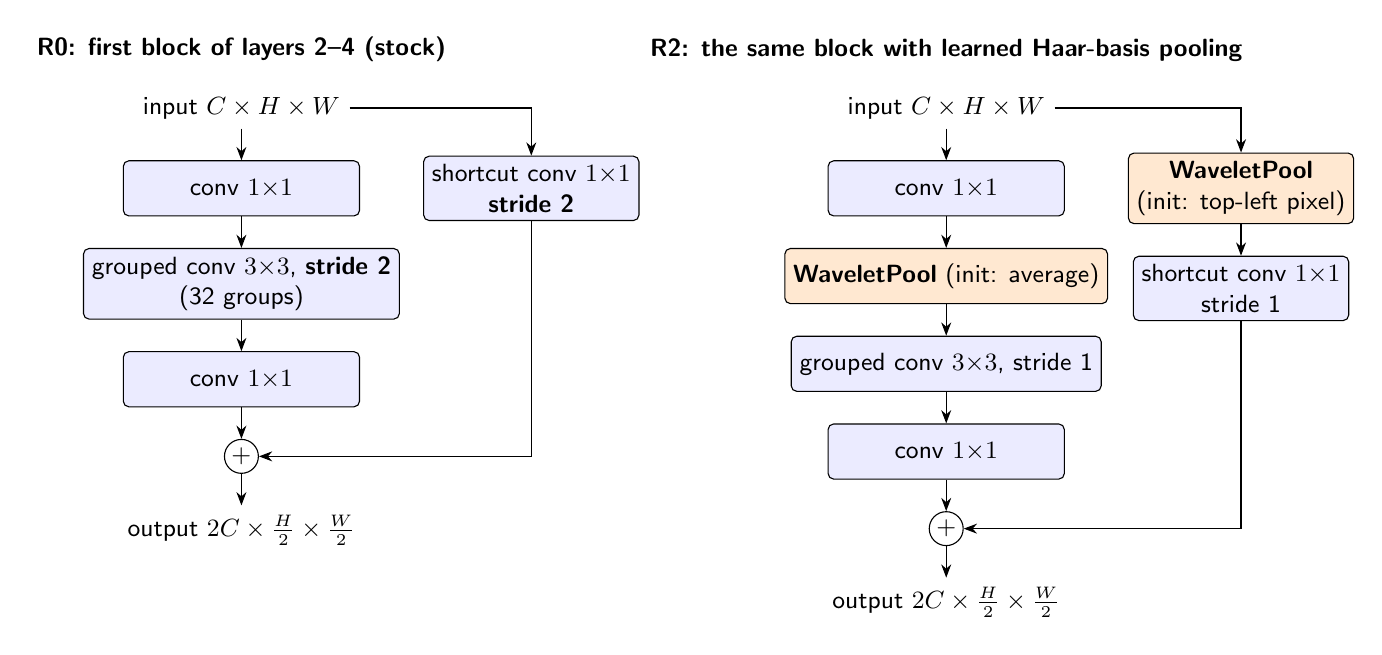
\begin{tikzpicture}[
  font=\sffamily\small, >=Stealth, node distance=4mm and 6mm,
  b/.style={draw, rounded corners=2pt, align=center, inner sep=3pt, fill=blue!8, minimum width=30mm, minimum height=7mm},
  w/.style={draw, rounded corners=2pt, align=center, inner sep=3pt, fill=orange!18, minimum width=30mm, minimum height=7mm},
  t/.style={align=center, font=\sffamily\small},
  title/.style={font=\sffamily\bfseries\small}]
% R0 block
\node[t] (in0) {input $C\times H\times W$};
\node[b, below=of in0] (a0) {conv $1{\times}1$};
\node[b, below=of a0] (g0) {grouped conv $3{\times}3$, \textbf{stride 2}\\(32 groups)};
\node[b, below=of g0] (e0) {conv $1{\times}1$};
\node[b, right=8mm of a0, minimum width=26mm] (s0) {shortcut conv $1{\times}1$\\\textbf{stride 2}};
\node[circle, draw, below=of e0, inner sep=1pt] (p0) {$+$};
\node[t, below=of p0] (o0) {output $2C\times\frac H2\times\frac W2$};
\draw[->] (in0) -- (a0); \draw[->] (a0) -- (g0); \draw[->] (g0) -- (e0); \draw[->] (e0) -- (p0); \draw[->] (p0) -- (o0);
\draw[->] (in0) -| (s0); \draw[->] (s0) |- (p0);
\node[title, above=2mm of in0] {R0: first block of layers 2--4 (stock)};
% R2 block
\node[t, right=62mm of in0] (in1) {input $C\times H\times W$};
\node[b, below=of in1] (a1) {conv $1{\times}1$};
\node[w, below=of a1] (wp1) {\textbf{WaveletPool} (init: average)};
\node[b, below=of wp1] (g1) {grouped conv $3{\times}3$, stride 1};
\node[b, below=of g1] (e1) {conv $1{\times}1$};
\node[w, right=8mm of a1, minimum width=26mm] (ws1) {\textbf{WaveletPool}\\(init: top-left pixel)};
\node[b, below=of ws1, minimum width=26mm] (s1) {shortcut conv $1{\times}1$\\stride 1};
\node[circle, draw, below=of e1, inner sep=1pt] (p1) {$+$};
\node[t, below=of p1] (o1) {output $2C\times\frac H2\times\frac W2$};
\draw[->] (in1) -- (a1); \draw[->] (a1) -- (wp1); \draw[->] (wp1) -- (g1); \draw[->] (g1) -- (e1); \draw[->] (e1) -- (p1); \draw[->] (p1) -- (o1);
\draw[->] (in1) -| (ws1); \draw[->] (ws1) -- (s1); \draw[->] (s1) |- (p1);
\node[title, above=2mm of in1] {R2: the same block with learned Haar-basis pooling};
\end{tikzpicture}
\end{document}
